\documentclass[chi_draft]{sigchi}

% Use this section to set the ACM copyright statement (e.g. for
% preprints).  Consult the conference website for the camera-ready
% copyright statement.

% Copyright
\CopyrightYear{2017}
%\setcopyright{acmcopyright}
\setcopyright{acmlicensed}
%\setcopyright{rightsretained}
%\setcopyright{usgov}
%\setcopyright{usgovmixed}
%\setcopyright{cagov}
%\setcopyright{cagovmixed}
% DOI
\doi{} %http://dx.doi.org/10.475/123_4}
% ISBN
\isbn{} %123-4567-24-567/08/06}
%Conference
\conferenceinfo{IoT'17,}{October 22--25, 2017, Linz, Austria}
%Price
\acmPrice{\$15.00}

% Use this command to override the default ACM copyright statement
% (e.g. for preprints).  Consult the conference website for the
% camera-ready copyright statement.

%% HOW TO OVERRIDE THE DEFAULT COPYRIGHT STRIP --
%% Please note you need to make sure the copy for your specific
%% license is used here!
% \toappear{
% Permission to make digital or hard copies of all or part of this work
% for personal or classroom use is granted without fee provided that
% copies are not made or distributed for profit or commercial advantage
% and that copies bear this notice and the full citation on the first
% page. Copyrights for components of this work owned by others than ACM
% must be honored. Abstracting with credit is permitted. To copy
% otherwise, or republish, to post on servers or to redistribute to
% lists, requires prior specific permission and/or a fee. Request
% permissions from \href{mailto:Permissions@acm.org}{Permissions@acm.org}. \\
% \emph{CHI '16},  May 07--12, 2016, San Jose, CA, USA \\
% ACM xxx-x-xxxx-xxxx-x/xx/xx\ldots \$15.00 \\
% DOI: \url{http://dx.doi.org/xx.xxxx/xxxxxxx.xxxxxxx}
% }

% Arabic page numbers for submission.  Remove this line to eliminate
% page numbers for the camera ready copy
% \pagenumbering{arabic}

% Load basic packages
\usepackage{balance}       % to better equalize the last page
\usepackage{graphics}      % for EPS, load graphicx instead 
\usepackage[T1]{fontenc}   % for umlauts and other diaeresis
\usepackage{txfonts}
\usepackage{mathptmx}
\usepackage[pdflang={en-US},pdftex]{hyperref}
\usepackage{color}
\usepackage{booktabs}
\usepackage{textcomp}

% Some optional stuff you might like/need.
\usepackage{microtype}        % Improved Tracking and Kerning
% \usepackage[all]{hypcap}    % Fixes bug in hyperref caption linking
\usepackage{ccicons}          % Cite your images correctly!
% \usepackage[utf8]{inputenc} % for a UTF8 editor only

% Custom packages

\usepackage{tikz}
\usetikzlibrary{shadows,shapes}
\usepackage{pgfplots}
\pgfplotsset{compat=1.10}

\usepackage{xcolor}
\usepackage{colortbl}
\definecolor{Gray}{gray}{0.90}

\usepackage{algorithm}
\usepackage{algorithmicx}
\usepackage{algpseudocode}

% If you want to use todo notes, marginpars etc. during creation of
% your draft document, you have to enable the "chi_draft" option for
% the document class. To do this, change the very first line to:
% "\documentclass[chi_draft]{sigchi}". You can then place todo notes
% by using the "\todo{...}"  command. Make sure to disable the draft
% option again before submitting your final document.
\usepackage[textsize=small]{todonotes}
\newcommand{\TODO}[1]{\todo[inline]{#1}}

% Paper metadata (use plain text, for PDF inclusion and later
% re-using, if desired).  Use \emtpyauthor when submitting for review
% so you remain anonymous.
\def\plaintitle{Private Blockchains for Transactive Energy:\\Security, Privacy, and Safety}
\def\plainauthor{First Author, Second Author, Third Author}
\def\emptyauthor{}
\def\plainkeywords{Internet of Things; blockchain; transactive energy; privacy; security; transactive microgrid.}
\def\plaingeneralterms{Design, Human Factors, Reliability, Security} % TODO: revise

% llt: Define a global style for URLs, rather that the default one
\makeatletter
\def\url@leostyle{%
  \@ifundefined{selectfont}{
    \def\UrlFont{\sf}
  }{
    \def\UrlFont{\small\bf\ttfamily}
  }}
\makeatother
\urlstyle{leo}

% To make various LaTeX processors do the right thing with page size.
\def\pprw{8.5in}
\def\pprh{11in}
\special{papersize=\pprw,\pprh}
\setlength{\paperwidth}{\pprw}
\setlength{\paperheight}{\pprh}
\setlength{\pdfpagewidth}{\pprw}
\setlength{\pdfpageheight}{\pprh}

% Make sure hyperref comes last of your loaded packages, to give it a
% fighting chance of not being over-written, since its job is to
% redefine many LaTeX commands.
\definecolor{linkColor}{RGB}{6,125,233}
\hypersetup{%
  pdftitle={\plaintitle},
% Use \plainauthor for final version.
%  pdfauthor={\plainauthor},
  pdfauthor={\emptyauthor},
  pdfkeywords={\plainkeywords},
  pdfdisplaydoctitle=true, % For Accessibility
  bookmarksnumbered,
  pdfstartview={FitH},
  colorlinks,
  citecolor=black,
  filecolor=black,
  linkcolor=black,
  urlcolor=linkColor,
  breaklinks=true,
  hypertexnames=false
}

% create a shortcut to typeset table headings
% \newcommand\tabhead[1]{\small\textbf{#1}}

% End of preamble. Here it comes the document.
\begin{document}

\title{\plaintitle}

\numberofauthors{3}
\author{%
  \alignauthor{Leave Authors Anonymous\\
    \affaddr{for Submission}\\
    \affaddr{City, Country}\\
    \email{e-mail address}}\\
  \alignauthor{Leave Authors Anonymous\\
    \affaddr{for Submission}\\
    \affaddr{City, Country}\\
    \email{e-mail address}}\\
  \alignauthor{Leave Authors Anonymous\\
    \affaddr{for Submission}\\
    \affaddr{City, Country}\\
    \email{e-mail address}}\\
}

\maketitle

\begin{abstract}
We design a secure and efficient trading platform for transactive microgrids, which enables prosumers to trade energy without sacrificing their privacy.
\end{abstract}

% TODO!
\category{K.6.m}{Miscellaneous}{Security}
\category{D.4.7}{Organization and Design}{Distributed systems}

\keywords{\plainkeywords}

\section{Introduction}

In order to take advantage of these capabilities, electric grids need to become more decentralized.

%However, simply broadcasting these bids would be catastrophic for privacy, since all the prosumers within a microgrid would learn of each others' expected consumption and production.

Transactive energy may pose a much greater threat to prosumers' privacy than smart metering.
\begin{itemize}
\item Firstly, since prosumers may purchase energy from each other in a transactive microgrid, transactions may inadvertently reveal the prosumers' detailed energy usage patterns to other prosumers within the microgrid.
Addressing this issue in a decentralized trading platform is quite challenging as it requires hiding the identities of trade partners from each other.
In comparison, secure smart metering reveals the prosumers' energy usage patterns only to the provider. 
\item Secondly, transactions may reveal the future energy usage of a prosumer, which could be used to infer private information.
For example, a smart home may know that its inhabitants will go out in the evening (e.g., by looking at their calendar), and it may trade energy futures accordingly in the morning.
Without adequate privacy measures, these trades may reveal to other prosumers in the microgrid that the inhabitants will not be at home later.
Note that energy futures, whose delivery may happen several hours after when the transaction is made, can play a very important role in predicting and controlling microgrid load.
In comparison, smart metering reveals only current (and past) usage.
\item Thirdly, transactions and energy usage data in a transactive microgrid are much richer source of information than the simple energy usage data collected by smart meters.
More specifically, the information available in a transactive microgrid is a superset of what is available from smart metering, and it may be used to infer personal information, such as risk propensity and financial standing.
\end{itemize}

\section{Solution Approaches}

\begin{figure*}[h]
\center
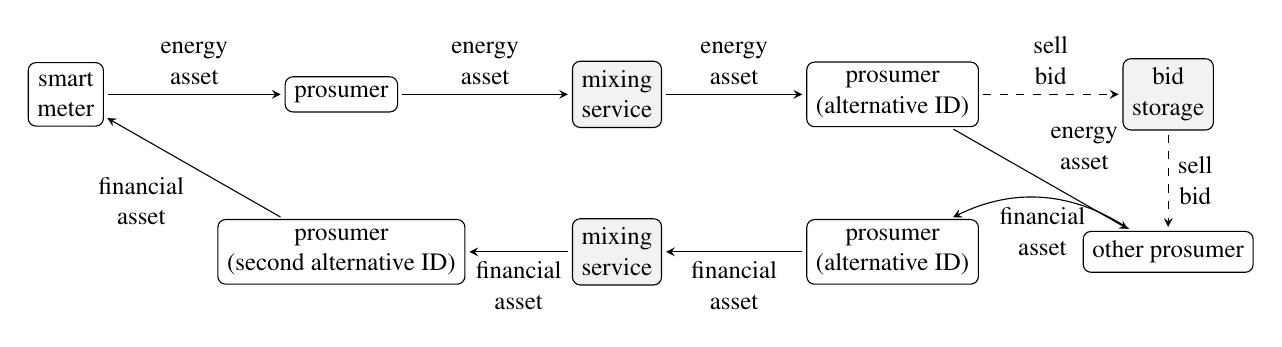
\begin{tikzpicture}[x=3.5cm, y=2cm, font=\small,
  system/.style={draw, align=center, rounded corners=0.1cm, fill=black!5},
  entity/.style={draw, align=center, rounded corners=0.1cm},
  asset/.style={midway, align=center},
  transfer/.style={->, >=stealth, shorten <=0.05cm, shorten >=0.05cm},
]
\node[entity] (smartmeter) at (0, 1) {smart\\meter};
\node[entity] (prosumer1) at (1, 1) {prosumer};
\node[system] (mixing1) at (2, 1) {mixing\\service};
\node[entity] (prosumer2) at (3, 1) {prosumer\\(alternative ID)};
\node[system] (bidstorage) at (4, 1) {bid\\storage};
\node[entity] (partner) at (4, 0) {other prosumer};
\node[entity] (prosumer3) at (3, 0) {prosumer\\(alternative ID)};
\node[system] (mixing2) at (2, 0) {mixing\\service};
\node[entity] (prosumer4) at (1, 0) {prosumer\\(second alternative ID)};


\draw[transfer] (smartmeter) -- node [asset, above] {energy\\asset} (prosumer1);
\draw[transfer] (prosumer1) -- node [asset, above] {energy\\asset} (mixing1);
\draw[transfer] (mixing1) -- node [asset, above] {energy\\asset} (prosumer2);
\draw[transfer, dashed] (prosumer2) -- node [asset, above] {sell\\bid} (bidstorage);
\draw[transfer, dashed] (bidstorage) -- node [asset, right] {sell\\bid} (partner);
\draw[transfer, bend right] (partner) to node [asset, below] {financial\\asset} (prosumer3);
\draw[transfer] (prosumer2) -- node [asset, above right] {energy\\asset} (partner);
\draw[transfer] (prosumer3) -- node [asset, below] {financial\\asset} (mixing2);
\draw[transfer] (mixing2) -- node [asset, below] {financial\\asset} (prosumer4);
\draw[transfer] (prosumer4) -- node [asset, below left] {financial\\asset} (smartmeter);
\end{tikzpicture}
\caption{Simplified overview of transactions for selling energy. Note that in order to prevent de-anonymization, a prosumer should use multiple addresses for mixing.}
\end{figure*}


\subsection{Communication Anonymity}
Firstly, we must provide an anonymous communication layer, on which we can build an anonymous trading platform.
Without this communication layer, bids and transactions could be easily de-anonymized based on the network identifiers of the sources (e.g., IP or MAC addresses).

We can employ well-known and widely used techniques for anonymous communication, such as \emph{onion routing}.
To build an onion network, the smart meters, inverters, and other devices can act as onion routers, and the list of onion routers in a microgrid can be published on a private blockchain.
In our first implementation, we can use the free and open-source Tor software with private Directory Authorities.
% ritter.vg: "run your own tor network"
% https://ritter.vg/blog-run_your_own_tor_network.html

\subsection{Transaction Anonymity}
We must provide prosumers with the ability to create and publish transactions anonymously.
More specifically, prosumers should be able to purchase or sell energy without revealing their identity; however, these transaction must also be verifiable and enforceable.

We may achieve this goal using multiple approaches for blockchain transaction anonymity:
\begin{itemize}
\item Mixing services (also known as tumblers) mix potentially identifiable assets on a blockchain with others, thereby preventing tracing individual assets back to their original source. 
In our case, assets to be mixed can include virtual balances of both fiat currencies and energy.
\item Cryptographic anonymity for transactions is provided, for example, by Zerocoin~\cite{miers2013zerocoin}. Similarly to mixing service, Zerocoin can prevent tracing assets on a blockchain.
\end{itemize}
Using the above techniques, we can enable prosumers to trade energy anonymously (i.e., without revealing their true identities), but at the same time prevent them from altering their energy or financial balances without a valid transaction.

However, 

\subsection{Bidding Anonymity}
Finally, we must provide prosumers with the ability to publish energy buy and sell bids anonymously.
To this end, we create a storage for anonymous bids that is readable by all the prosumers in the microgrid.
Any prosumer may submit a bid to this storage; however, in order to do so, they must provide a zero-knowledge proof of owning the assets that are to be traded:
\begin{itemize}
\item To submit an energy sell bid, the prosumer must prove that it owns an energy production asset on the chain.
\item To submit an energy buy bid, the prosumer must prove that it own an energy consumption asset as well as financial assets on the chain.
\end{itemize}


\section{Related Work}

\subsection{Smart Grid and Meter Privacy}



\subsection{Blockchain Technology}

Microsoft offers Blockchain as a Service (BaaS) on Azure.
Project Bletchley is Microsoft's architectural approach to building an Enterprise Consortium Blockchain Ecosystem, introducing two new concepts: blockchain middleware and cryptlets~\cite{gray2016introducing}.

Hyperledger Fabric is a platform for distributed ledger solutions, which was designed to support pluggable implementations of different components~\cite{hyperledger2017fabric}.

Interledger is a protocol for payments across payment systems, which enables anyone with accounts on two ledgers to create
a connection between them~\cite{thomas_protocol}.

Bitcoin Lightning Network is decentralized system, in which transactions are sent over a network of micropayment channels whose transfer of value occurs off-blockchain~\cite{poon2016bitcoin}.

\url{https://geli.net/residential/}
\url{https://www.greentechmedia.com/articles/read/geli-raises-7m-to-take-energy-storage-software-to-the-next-level}






% BALANCE COLUMNS
\balance{}

% REFERENCES FORMAT
% References must be the same font size as other body text.
\bibliographystyle{SIGCHI-Reference-Format}
\bibliography{references}

\clearpage
\appendix

\section{Architecture Overview}

\begin{figure}[h!]
\center
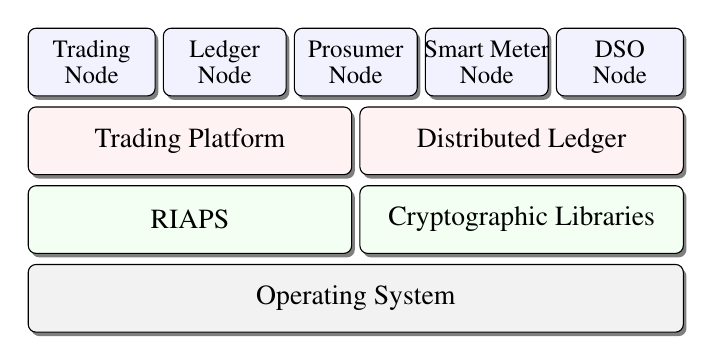
\begin{tikzpicture}[
  x=1.04cm,
  nodeStyle/.style={rounded corners=0.1cm, drop shadow={shadow xshift=0.04cm, shadow yshift=-0.05cm, fill=black}}]
  
\draw [fill=blue!5, nodeStyle] (0, 3.07) rectangle (1.55, 3.93) node [midway, align=center, font=\small] {Trading\\[-0.2em]Node};
\draw [fill=blue!5, nodeStyle] (1.65, 3.07) rectangle (3.15, 3.93) node [midway, align=center, font=\small] {Ledger\\[-0.2em]Node};
\draw [fill=blue!5, nodeStyle] (3.25, 3.07) rectangle (4.75, 3.93) node [midway, align=center, font=\small] {Prosumer\\[-0.2em]Node};
\draw [fill=blue!5, nodeStyle] (4.85, 3.07) rectangle (6.35, 3.93) node [midway, align=center, font=\small] {Smart Meter\\[-0.2em]Node};
\draw [fill=blue!5, nodeStyle] (6.45, 3.07) rectangle (8.0, 3.93) node [midway, align=center, font=\small] {DSO\\[-0.2em]Node};

\draw [fill=red!5, nodeStyle] (0, 2.07) rectangle (3.95, 2.93) node [midway] {Trading Platform};
\draw [fill=red!5, nodeStyle] (4.05, 2.07) rectangle (8, 2.93) node [midway] {Distributed Ledger};

\draw [fill=green!5, nodeStyle] (0, 1.07) rectangle (3.95, 1.93) node [midway] {RIAPS};
\draw [fill=green!5, nodeStyle] (4.05, 1.07) rectangle (8, 1.93) node [midway] {Cryptographic Libraries};

\draw [fill=black!5, nodeStyle] (0, 0.07) rectangle (8, 0.93) node [midway] {Operating System};
\end{tikzpicture}
\caption{High-level software architecture.}
\label{fig:softwareArchitecture}
\end{figure}

Figure~\ref{fig:softwareArchitecture} shows a high-level overview of the software architecture of our system.
Our system is -- in part -- built on the Resilient Information Architecture for Smart Grid (RIAPS) platform~\cite{eisele2017riaps}.

Figure~\ref{fig:logicalNodeArchitecture} shows a high-level overview of the trading platform, the distributed ledger, and the logical nodes implementing and interacting with these subsystems.

\paragraph{Trading Platform}
Although individual prosumers trade energy with each other, for the sake of scalability, we need a trading platform that enables prosumers to find trade partners.
By serving as a database for energy bids, the trading platform relieves prosumer nodes from communicating with all potential trade partners.~%
\footnote{Note that prosumers are not required to use the services of the trading platform, and they are allowed to communicate with each other for the sake of finding trade partners.
However, in a microgrids with a large number prosumers, the trading platform will be able to find partners more efficiently and promptly.}
In addition to receiving and storing bids from prosumers, the trading platform can also find matches and notify the prosumers of the opportunity to make an energy trade.
Even though the trading platform appears to the nodes as one entity, for the sake of scalability and reliability, it can be implemented in a distributed manner, using multiple trading nodes.

\paragraph{Distributed Ledger}
The distributed ledger stores transactions that specify energy trades, record energy production and consumption, and change regulatory policies for the microgrid, including energy prices.
Since the ledger is maintained by multiple ledger nodes, a key implementation requirement is reaching consensus on which transactions are valid and stored in the ledger.
This consensus must be reached quickly, reliably, and securely even in the presence of erroneous or even malicious ledger nodes.
We treat the consensus algorithm as a pluggable module, which can be based on blockchains with proof-of-stake consensus or Practical Byzantine Fault Tolerance algorithm~\cite{castro1999practical}.

\paragraph{Controller}
The controller is responsible for stabilizing load within the microgrid and controlling it based on the expected load in the rest of the grid.
To this end, the controller first estimates the expected load in the microgrid based on outstanding energy trades on the ledger.
By combining this estimate with the expected load in the remainder of the grid, the controller produces a control signal that specifies how much the load in the microgrid needs to be decreased or increased.
Finally, based on this control signal, the controller updates the price policy for the microgrid to influence energy production and consumption.
The controller may be implemented by the DSO node, as part of the RIAPS-based platform, or may be a legacy controller that interfaces with the DSO node.

\begin{figure*}
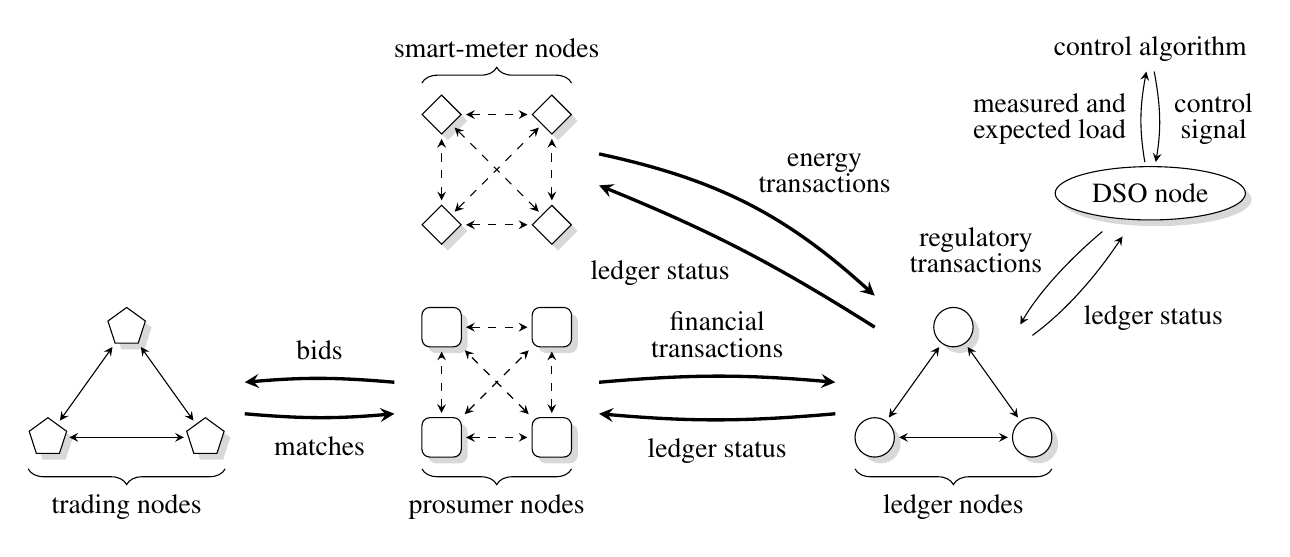
\begin{tikzpicture}[
  x=1cm, 
  y=1cm,
  nodeStyle/.style={fill=white, draw=black, drop shadow=black!30, minimum size=0.5cm},
  linkStyle/.style={<->, >=stealth, shorten >=1.5pt, shorten <=1.5pt},
  batchStyle/.style={->, very thick, >=stealth},
  braceStyle/.style={decorate, decoration={brace,amplitude=0.2cm}, yshift=-0.4cm},
]

% trading nodes
\begin{scope}[xshift=1cm]

\foreach \name/\x/\y in {{t1/0/0}, {t2/1/1.4}, {t3/2/0}}
  \node [nodeStyle, regular polygon, regular polygon sides=5] (\name) at (\x,\y) {};

\foreach \name/\x/\y in {{tRight/2.5/0.7}}
  \coordinate (\name) at (\x,\y);

\foreach \from/\to in {{t1/t2}, {t2/t3}, {t3/t1}}
  \draw [linkStyle] (\from) -- (\to);
  
\draw [braceStyle] (2.25, 0) -- (-0.25, 0) node [midway, below=0.2cm] {trading nodes};
\end{scope}

% prosumer nodes
\begin{scope}[xshift=6cm]

\foreach \name/\x/\y in {{p1/0/0}, {p2/1.4/0}, {p3/0/1.4}, {p4/1.4/1.4}}
  \node [nodeStyle, rounded corners=0.1cm] (\name) at (\x,\y) {};

\foreach \name/\x/\y in {{pLeft/-0.6/0.7}, {pRight/2/0.7}}
  \coordinate (\name) at (\x,\y);

\foreach \from/\to in {{p1/p2}, {p1/p3}, {p1/p4}, {p2/p3}, {p2/p4}, {p3/p4}}
  \draw [linkStyle, dashed] (\from) -- (\to);
  
\draw [braceStyle] (1.65, 0) -- (-0.25, 0) node [midway, below=0.2cm] {prosumer nodes};
\end{scope}

% smart-meter nodes
\begin{scope}[xshift=6cm, yshift=2.7cm]

\foreach \name/\x/\y in {{m1/0/0}, {m2/1.4/0}, {m3/0/1.4}, {m4/1.4/1.4}}
  \node [diamond, nodeStyle] (\name) at (\x,\y) {};

\foreach \name/\x/\y in {{mRight/2/0.7}}
  \coordinate (\name) at (\x,\y);

\foreach \from/\to in {{m1/m2}, {m1/m3}, {m1/m4}, {m2/m3}, {m2/m4}, {m3/m4}}
  \draw [linkStyle, dashed] (\from) -- (\to);
  
\draw [braceStyle, yshift=0.8cm] (-0.25, 1.4) -- (1.65, 1.4) node [midway, above=0.2cm] {smart-meter nodes};
\end{scope}

% ledger nodes
\begin{scope}[xshift=11.5cm]

\foreach \name/\x/\y in {{l1/0/0}, {l2/1/1.4}, {l3/2/0}}
  \node [circle, nodeStyle] (\name) at (\x,\y) {};

\foreach \name/\x/\y in {{lLeft/-0.5/0.7}, {lTopLeft/0/1.6}, {lTopRight/1.6/1.0}}
  \coordinate (\name) at (\x,\y);

\foreach \from/\to in {{l1/l2}, {l2/l3}, {l3/l1}}
  \draw [<->, >=stealth, shorten >=1.5pt, shorten <=1.5pt] (\from) -- (\to);
  
\draw [decorate, decoration={brace,amplitude=0.2cm}, yshift=-0.4cm] (2.25, 0) -- (-0.25, 0) node [midway, below=0.2cm] {ledger nodes};
\end{scope}

% additional nodes
\node [ellipse, nodeStyle] (dso) at (15cm, 3.1cm) {DSO node};

\draw [->, >=stealth, bend right=10, shorten <=0.25cm, shorten >=0.5cm] (dso) to node [midway, above left=0cm, align=center] {regulatory\\[-0.25em]transactions} (lTopRight);
\draw [<-, >=stealth, bend left=10, shorten <=0.25cm, shorten >=0.5cm] (dso) to node [midway, below right=0cm, align=center] {ledger status} (lTopRight);

\node [above=1.2cm of dso] (controller) {control algorithm}; 

\draw [<-, >=stealth, bend right=10, shorten <=1.5pt] (dso) to node [midway, left=0.3cm, align=center] {measured and\\[-0.25em]expected load} (controller);
\draw [->, >=stealth, bend left=10, shorten <=1.5pt] (dso) to node [midway, right=0.3cm, align=center] {control\\[-0.25em]signal} (controller);

% connections between systems
\draw [batchStyle, <-, bend left=5] (tRight) to node [midway, above=0.1cm] {bids} (pLeft);
\draw [batchStyle, bend right=5] ([yshift=-0.4cm]tRight) to node [midway, below=0.1cm] {matches} ([yshift=-0.4cm]pLeft);

\draw [batchStyle, bend left=5] (pRight) to node [midway, above=0.1cm, align=center] {financial\\[-0.25em]transactions} ([yshift=0cm]lLeft);
\draw [batchStyle, <-, bend right=5] ([yshift=-0.4cm]pRight) to node [midway, below=0.1cm] {ledger status} ([yshift=-0.4cm]lLeft);

\draw [batchStyle, bend left=15] ([yshift=0.2cm]mRight) to node [midway, above right=0cm, align=center] {energy\\[-0.25em]transactions} ([yshift=0.2cm]lTopLeft);
\draw [batchStyle, <-, bend right=-5] ([yshift=-0.2cm]mRight) to node [midway, below left=0cm] {ledger status} ([yshift=-0.2cm]lTopLeft);

\end{tikzpicture}
\caption{High-level logical architecture of the trading platform and the distributed ledger. A physical node may implement multiple logical nodes.}
\label{fig:logicalNodeArchitecture}
\end{figure*}



\subsection{Timing}

Timing is a crucial part of our platform.
For example, control signals specify how the load should change at certain points in time, energy trades specify when energy will be consumed or produced, etc.
To facilitate processing signals and transactions, we divide time into fixed-length intervals, and specify points or periods in time using these discrete time intervals.
The length of the time interval is determined by mapping the timing assumptions of the power system to our platform.
In our implementation, for example, the default length of the time interval is 4 seconds, which corresponds to how frequently the control signal of the DSO changes.

\begin{figure}[h!]
\center
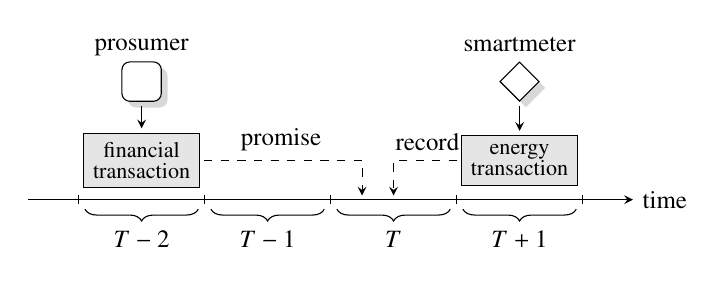
\begin{tikzpicture}[
  x=1.6cm,
  font=\small,
  nodeStyle/.style={fill=white, draw=black, drop shadow=black!30, minimum size=0.5cm},
  arrowStyle/.style={->, >=stealth, shorten >=1.5pt, shorten <=1.5pt},
  transactionStyle/.style={draw, align=center, fill=black!10, font=\footnotesize}]
\draw [->, >=stealth] (0.6, 0) -- (5.4, 0) node [right] {time};

\foreach \pos in {1, 2, 3, 4, 5}
  \draw (\pos, 0.06cm) -- (\pos, -0.06cm);
  
\foreach \pos/\name in {{1/$T-2$}, {2/$T-1$}, {3/$T$}, {4/$T+1$}}
  \draw[decorate, decoration={brace,amplitude=0.15cm}, yshift=-0.12cm] ({\pos+0.95}, 0) -- ({\pos+0.05}, 0) node [midway, below=0.15cm, font=\small] {\name};
  
\node [nodeStyle, rounded corners=0.1cm] (prosumer) at (1.5, 1.5) {};
\node [nodeStyle, diamond] (smartmeter) at (4.5, 1.5) {};

\node [above=-0.05cm of prosumer] {prosumer};
\node [above=0cm of smartmeter] {smartmeter};

\node [transactionStyle] (financial) at (1.5, 0.5) {financial\\[-0.25em]transaction};
\node [transactionStyle] (energy) at (4.5, 0.5) {energy\\[-0.25em]transaction};

\draw [arrowStyle] (prosumer) -- (financial);
\draw [arrowStyle] (smartmeter) -- (energy);

\draw [arrowStyle, dashed] (financial) -- (3.25, 0.5) node [midway, above] {promise} -- (3.25, 0);
\draw [arrowStyle, dashed] (energy) -- (3.5, 0.5) node [midway, above] {record} -- (3.5, 0);
\end{tikzpicture}
\caption{Basic timeline of transactions.}
\label{fig:timeline}
\end{figure}

All transactions for energy trading are specified with respect to these discrete intervals: financial transactions promise to consume or produce a certain amount of energy in a future interval, while energy transactions record the actual amount of energy produced or consumed in an earlier interval. 
Figure~\ref{fig:timeline} shows a basic timeline of financial and energy transactions.

\begin{table*}
\center
\caption{Logical Node Types}
\label{tab:logicalNodeTypes}
\begin{tabular}{|c||p{4.6cm}|l|l|}
\hline
\textbf{Type} & \textbf{Function} & \textbf{Cardinality} & \textbf{Physical node} \\
\hline\hline
\rowcolor{Gray} Ledger      & maintain distributed ledger                 & one or more           & any node (with enough computational power) \\ \hline
                Trading     & provide trading platform                    & one or more           & any node (with enough computational power) \\ \hline
\rowcolor{Gray} Prosumer    & trade electricity (on behalf of a prosumer) & one for each prosumer & smart inverter or smart meter \\ \hline
                Smart meter & record power consumption and production     & one for each prosumer & smart meter (must be trusted hardware) \\ \hline
\rowcolor{Gray} DSO         & regulate microgrid electricity market       & one                   & node owned by the DSO \\ \hline
\end{tabular}
\end{table*}

\subsection{Logical Nodes}

Next, we discuss the five types of logical nodes in our system: ledger, trading, prosumer, smart meter, and DSO nodes.
Table~\ref{tab:logicalNodeTypes} shows an overview of these logical-node types.

Every node has a pair of public and private keys as well as a digital certificate from the DSO, which proves the ownership of the public key.
The nodes can use the key pair and the certificate to prove their identity and to sign messages or transactions.
A digital certificate may also specify the capabilities of a node.
For example, the certificate of a prosumer node may specify the amount of energy that the node is allowed to trade for a single time interval.
% physical node certificates may also describe roles that may be taken by the physical node
% In addition to capabilities, the certificate may also describe roles, that is, logical nodes that can be implemented by the physical node.

\subsubsection{Ledger nodes}
Ledger nodes implement the distributed ledger by forming a peer-to-peer network with each other and reaching a consensus on the state of the ledger.
A ledger node is responsible for receiving financial transactions from prosumer nodes, energy transactions from smart-meter nodes, and regulatory transactions from the DSO node.
The ledger nodes share these transactions with each other, verify them, and reach a consensus on which transactions are recorded in the ledger. 

\subsubsection{Trading nodes}
Trading nodes implement the distributed trading platform by forming a peer-to-peer network with each other and providing services for prosumer nodes.
A trading node is responsible for receiving bids from prosumer nodes, sharing these bids with the other trading nodes, maintaining a distributed database of active bids, trying to match bids with each other, and notifying the prosumers of matches.
While this platform is similar to the distributed ledger in many ways, it is subject to much less stringent requirements.
For example, the trading platform does not have to store history in a reliable and verifiable manner.
Consequently, trading nodes can be implemented by computationally less capable physical nodes (e.g., with limited storage).

\begin{table*}
\center
\caption{Transaction Types}
\label{tab:transactionTypes}
\begin{tabular}{|c||l|l|p{5cm}|}
\hline
\textbf{Type} & \textbf{Creator} & \textbf{Contents} & \textbf{Validity} \\
\hline\hline
\rowcolor{Gray} Financial  & prosumers    & identifiers, signatures, time interval, amount of energy & signed by buyer and seller, abides by the safety and security rules \\ \hline
                Energy     & smart meters & identifier, signature, time interval, amount of energy   & signed by smart meter \\ \hline
\rowcolor{Gray} Regulatory & DSO          & signature, time interval, set of policy updates            & signed by DSO \\ \hline
\end{tabular}
\end{table*}

\subsubsection{Prosumer nodes}
Each prosumer node represents a prosumer, such as a residential customer.
A prosumer node trades future electricity consumption and production on behalf of the prosumer.
As a first step in electricity trading, the prosumer node estimates the net energy demand of the prosumer for a future time interval.
At the same time, it queries the active regulatory policies, such as energy prices, from the distributed ledger.
Based on the estimated net demand and the active regulatory policies, it creates an energy trading bid, which it then submits to the trading platform.
If the trading platform responds with one (or more) matching bid, then the prosumer node contacts the node that submitted a matching bid.
The two nodes negotiate, agree on, create, and sign a new financial transaction, which they then submit to the distributed ledger.
\todo[inline]{Extend: prosumer nodes may buy/sell electricity from/to DSO in advance. This is key to load prediction.}
Once the ledger has verified and recorded the transaction, the electricity trade has been set up.

\subsubsection{Smart-meter nodes}
Each smart-meter node measures the actual energy production and consumption of a prosumer.
For each time interval, the smart-meter node measures the net energy consumption of the prosumer, records the net consumption in an energy transaction, and then signs the transaction and submits it to the distributed ledger.
To ensure that the smart-meter node measures the correct amount of net consumption, the node must always be implemented by a trusted smart meter deployed at the prosumer.
Furthermore, we assume that the smart-meter devices are tamper-proof hardware, which prevents tampering attacks by the prosumers (e.g., to avoid paying for electricity).

\subsubsection{DSO node}
The DSO node represents the Distribution System Operator, and it is responsible for regulating the microgrid market using regulatory transactions.
These transactions enable the DSO, for example, to set a price policy for the microgrid or to remove misbehaving nodes by revoking their certificates.
Note that in order to enhance reliability and security, the DSO node may be split into multiple logical nodes.
For example, the DSO node can be split into a pricing node, which is authorized and responsible for setting the price policy, and a revocation node, which is authorized and responsible for revoking digital certificates.

\subsection{Transactions}

Transactions on the distributed ledger can be divided into three main types: financial, energy, and regulatory transactions.
Table~\ref{tab:transactionTypes} shows an overview of these transaction types.

\subsubsection{Financial Transactions}
A financial transaction represents an agreement between two prosumers, called the seller and the buyer, who promise to respectively produce and consume a certain amount of energy in a future time interval.

A financial transaction contains the following fields:
\todo[inline]{Extend: prosumer nodes may buy/sell electricity from/to DSO in advance. This is key to load prediction.}
\begin{itemize}
\item \textbf{Seller ID}: Unique identifier of the selling prosumer node.
\item \textbf{Buyer ID}: Unique identifier of the buying prosumer node.
\item \textbf{Monetary value}: Value paid by the buyer to the seller, which can be denominated in either a fiat currency (e.g., US dollars) or a cryptocurrency.
\item \textbf{Time interval}: Identifier of the time interval in which energy will be produced and consumed.
\item \textbf{Energy value}: Amount of energy produced by the seller and consumed by the buyer.
\item \textbf{Seller signature}: Digital signature created using the private key of the seller, computed over all previous fields.
\item \textbf{Buyer signature}: Digital signature created using the private key of the seller, computed over all previous fields except the seller signature.
\end{itemize}

The ledger nodes accept and record a financial transaction if
\begin{itemize}
\item both signatures are valid,
\item time interval is in the future,
\item transaction abides by the safety and security rules set by the DSO (we will discuss these rules in detail later).
\end{itemize}

\subsubsection{Energy Transactions}
An energy transaction records the actual amount of energy consumed and produced by a prosumer in a past time interval.

An energy transaction contains the following fields:
\begin{itemize}
\item \textbf{Smart-meter ID}: Unique identifier of the smart meter.
\item \textbf{Energy value}: Net amount of energy consumed by the prosumer, which is computed as the difference between the consumption and the production of the prosumer (note that it may be a negative value if the prosumer produced more than its consumption).
\item \textbf{Time interval}: Identifier of the time interval in which energy consumption and production were measured.
\item \textbf{Smart-meter signature}: Digital signature created using the private key of the smart meter, computed over all previous fields.
\end{itemize}

The ledger nodes accept and record an energy transaction if
\begin{itemize}
\item signature is valid
\item time interval is in the past.
\end{itemize}

\subsubsection{Regulatory Transactions}
A regulatory transaction changes the set of active policies which all transactions are subject to.
To provide elaborate tools for regulating a microgrid, our system may support a variety of intricate regulatory transactions.
Here, we discuss two transactions that are necessary for regulating any microgrid market: price-policy and certificate-revocation transactions.

\paragraph{Price policy}
A price-policy transaction changes the active price policy of the DSO for the microgrid.
A price policy specifies how much a prosumer will have to pay to the DSO for the difference between its promised and actual net consumption.

A price-policy transaction contains the following fields:
\begin{itemize}
\item \textbf{Time interval}: Identifier of the time interval from which the new price policy will be active.
\item \textbf{Price policy}: Specification of the new price policy.
\item \textbf{DSO signature}: Digital signature created using the private key of the DSO, computed over all previous fields.
\end{itemize}

The ledger nodes accept and record a price-policy transaction if
\begin{itemize}
\item signature is valid
\item time interval is in the future.
\end{itemize}

\paragraph{Certificate Revocation}
A certificate-revocation transaction revokes some of the digital certificates that were issued to the nodes.
After a certificate has been revoked, ledger nodes will no longer accept digital signatures created using key pairs whose ownership was proven by the certificate.

A certificate-revocation transaction contains the following fields:
\begin{itemize}
\item \textbf{Time interval}: Identifier of the time interval in which the certificate is revoked.
\item \textbf{List of certificates}: Certificates to be revoked.
\item \textbf{DSO signature}: Digital signature created using the private key of the DSO, computed over all previous fields.
\end{itemize}

The ledger nodes accept and record a certificate-revocation transaction if
\begin{itemize}
\item signature is valid
\item time interval is in the future.
\end{itemize}


\subsection{Privacy}

Depending on the level of privacy that must be provided, the proposed system may be implemented in multiple ways.
Here, we describe and discuss two approaches, called open and private systems, which are corner cases with respect to privacy.

\subsubsection{Open System}
This approach is aimed at cases when privacy within a microgrid is not a concern, and we can design the system to maximize its efficiency.
\begin{itemize}
\item We allow any physical node to become a trading or ledger node. This enhances reliability -- and potentially performance -- as the trading platform and distributed ledger can be implemented by a large set of physical nodes.
\item The distributed ledger is public within the microgrid, which means that any node can query and receive the complete list of validated and recorded transactions.
\end{itemize}
% Advantages: easier accountability and reliability

\subsubsection{Private System}
This approach is aimed at cases when privacy is a crucial requirement, for example, when the DSO and the microgrid are legally required to provide privacy.
% goal: hide any personal information
\begin{itemize}
\item We allow only a limited set of physical nodes to act as ledger or trading nodes. This constraint can be enforced through limiting the roles of a node within its certificate.
\item The distributed ledger is private. When a node queries the status of the ledger, it will only receive 1) regulatory transactions, 2) aggregate information regarding expected consumption and production in future time steps, 3) list of transactions in which the node is involved.
\end{itemize}
To further enhance security, we can also enable the trading platform to mediate between prosumers who would like to trade energy. With the help of the trading platform, two prosumer nodes can create a financial transaction without learning each other's identity, and this transaction can then be submitted to the ledger by the trading platform.


\subsection{Transaction Validation and Interpretation}

Here, we discuss the details of how to validate and interpret the financial and energy transactions.
First, we detail how the ledger nodes determine which transactions are valid and recorded in the distributed ledger.
Second, we explain how financial and energy transactions can be aggregated in order to determine the financial balance of a prosumer.

\subsubsection{Validation of Financial Transactions: Safety and Security}

First, the ledger nodes reach consensus on the order of the transactions that have been submitted for recording on the ledger.
Second, they reach consensus on the validity of the ordered transactions.
They determine the validity of the transactions one-by-one, making a decision for each transaction based on its contents and the contents of the preceding valid transactions.

To ensure the safety and security of the microgrid, ledger nodes must be able to reject careless or malicious energy trading, which could destabilize the microgrid.
To this end, the certificate of each prosumer specifies the net amount of energy that the prosumer may trade for a single time step.
More specifically, the certificate of prosumer $p$ includes the following fields:
\begin{itemize}
\item $MaxNetBuy_p$: net energy that prosumer $p$ may purchase,
\item $MaxNetSell_p$: net energy that prosumer $p$ may sell.
\end{itemize}

To determine whether an incoming financial transaction is valid, a ledger node runs Algorithm~\ref{alg:validateFinancialTransaction}.
%\begin{enumerate}
%\item let $T$ be the time step of the incoming transaction, and let $p_b$ and $p_s$ be the buying and selling prosumers, respectively;
%\item let $NetBuy \gets 0$;
%\item for every valid transaction on the ledger, if the time step is $T$ and the buyer is $p_b$, then add the energy amount to $NetBuy$;
%\item for every valid transaction on the ledger, if the time step is $T$ and the seller is $p_b$, then subtract the energy amount from $NetBuy$;
%\item let $NetSell \gets 0$;
%\item for every valid transaction on the ledger, if the time step is $T$ and the seller is $p_s$, then add the energy amount to $NetSell$;
%\item for every valid transaction on the ledger, if the time step is $T$ and the buyer is $p_s$, then subtract the energy amount from $NetSell$;
%\item if $NetBuy \leq MaxNetBuy_{p_b}$, $NetSell \leq MaxNetSell_{p_s}$, the signatures are valid, and $T$ is in the future, then output valid;
%\item else, output invalid.
%\end{enumerate}

\todo[inline]{Extend: prosumer nodes may buy/sell electricity from/to DSO in advance. This is key to load prediction.}

\begin{algorithm}[h!]
\caption{Validation of Financial Transaction}
\label{alg:validateFinancialTransaction}
\begin{algorithmic}[1]
\Statex{\hspace{-\algorithmicindent}\textbf{Input:} incoming transaction, valid transactions on the ledger}
\Statex{\hspace{-\algorithmicindent}\textbf{Output:} valid / invalid}
\State{let $T$ be the time step of the incoming transaction, and let $p_b$ and $p_s$ be the buying and selling prosumers, respectively}
\State{$NetBuy \gets 0$}
\State{$NetSell \gets 0$}
\For{valid transaction on the ledger}
  \If{time step is $T$}
    \If{buyer is $p_b$}
      \State{$NetBuy \gets NetBuy + $ energy amount}
    \EndIf
    \If{seller is $p_b$}
      \State{$NetBuy \gets NetBuy - $ energy amount}
    \EndIf
    \If{seller is $p_s$}
      \State{$NetSell \gets NetSell + $ energy amount}
    \EndIf
    \If{buyer is $p_s$}
      \State{$NetSell \gets NetSell - $ energy amount}
    \EndIf
  \EndIf
\EndFor
\If{$NetBuy \leq MaxNetBuy_{p_b}$, $NetSell \leq MaxNetSell_{p_s}$, the signatures are valid, and $T$ is in the future}
  \State{\textbf{return} valid}
\Else
  \State{\textbf{return} invalid}
\EndIf
%
%\State{$A \gets (\emptyset, \emptyset)$} 
%\State{$\Loss^* \gets -\infty$}
%\For{$b = 1, \ldots, B_A$}
%  \For{$v \in V_A$}
%    \For{$k \in \Gamma^{-1}(v)$}
%      \State{$A' \gets A \cup \left(\{s\}, \left\{\hat{p}_{kv} = 1, \forall j \neq k : \hat{p}_{jv} = 0\right\}\right)$}
%      \State{$\Loss' \gets \big[\left(1 - \Pr[\text{detect}]\right) \cdot \Loss(C, A)$}
%      \State{\hspace{3.5em} $+ \Pr[\text{detect}] \cdot \min_M \max_R \Loss(C, A, M, R) \big]$}
%      \If{$\Loss' \geq \Loss^*$}
%        \State{$A^* \gets A'$}
%        \State{$\Loss^* \gets \Loss'$}
%      \EndIf
%    \EndFor
%    \State{$A \gets A^*$}
%  \EndFor
%\EndFor
%\State{Output $A$}
\end{algorithmic}
\end{algorithm}

\subsubsection{Aggregation of Financial and Energy Transactions: Financial Balance}

\todo[inline]{Firstly, the prosumer must pay (or be paid) for the financial transactions recorded on the ledger in either a fiat currency (e.g., US dollars) or a cryptocurrency.}

Even though prosumer nodes attempt to buy or sell in advance the amount of energy that they will consume or produce, it is practically impossible to predict their net consumption perfectly.
Consequently, there will necessarily be an imbalance between the amount of energy bought (or sold) in advance and the actual net consumption (or production) of the prosumer.
This imbalance must be covered by the DSO, who will charge (or pay) the prosumer for the amount of energy consumed (or produced) beyond what was promised in the financial transactions.

The amount that the DSO will charge (or pay) the prosumer is determined by the pricing policy of the DSO, which is set using regulatory transactions.


\subsection{Control Algorithm}

\todo[inline]{
\textbullet 
receives measured and expected load values from the ledger (as well as from the rest of the grid)
\textbullet 
produces a control signal that specifies the desired load for the future (may also include a tolerance level that specifies how much deviation from this load level is tolerable)
}

\todo[inline]{Figure: - data flow between nodes - control signals}

\end{document}

